% ==============================================================================
% ACM 2-Column Conference Template (sigconf) — Skeleton Only (Zero AI Prose)
% Target Length: 6-8 pages (including references)
% Recommended Platform: Overleaf (select TeX Live 2023+ / pdflatex)
% ==============================================================================
\documentclass[sigconf,nonacm]{acmart}

% Clean course-project header/footer (removes fake ACM copyright block)
\settopmatter{printacmref=false}
\renewcommand\footnotetextcopyrightpermission[1]{}
\pagestyle{plain}

\usepackage{booktabs}
\usepackage{amsmath}
\usepackage{graphicx}
\usepackage{xcolor}
\usepackage{listings}

\lstset{
  basicstyle=\ttfamily\scriptsize,
  breaklines=true,
  frame=single,
  backgroundcolor=\color{gray!8}
}

\begin{document}

\title{Uncertainty-Gated Hybrid Cascade for Trust-Aware Credit Card Fraud Detection}
\subtitle{AI 630: Responsible Artificial Intelligence --- Course Project Final Paper}

\author{Hammad, Ammar, Daud, Rizwan, Sarmad}
\affiliation{%
  \institution{Syed Babar Ali School of Science and Engineering (SBASSE), LUMS}
  \city{Lahore}
  \country{Pakistan}
}

% ==============================================================================
% ABSTRACT (~150-200 words)
% ==============================================================================
\begin{abstract}
% TODO [WRITE IN YOUR OWN WORDS - 150-200 words]:
% 1. State the banking problem: tabular models fail silently under class imbalance (2.06% fraud) and drift, while LLMs (~1.43s/tx) are too slow for 100% of traffic.
% 2. Summarize your 2-tier cascade: System-1 (LightGBM + 20-pass MC Dropout CreditNet), Dual Gate (aleatoric margin + epistemic std), and System-2 (gemini-3.5-flash-lite).
% 3. Report headline numbers on N=16,707 test tx: 90.27% automated at 17.3 ms single-tx latency (0.406 ms batch-amortized), auto-slice ECE reduced to 0.0047, silent FN reduced 232 -> 168.
% 4. Mention live 40-case Gemini audit: 18/25 (72.0%; 85.7% non-timeout) legitimate clearance and discovery of LLM base-rate anchoring.
\end{abstract}

\keywords{Trust-Aware Machine Learning, Credit Card Fraud Detection, Uncertainty Quantification, Selective Classification, Monte Carlo Dropout, Large Language Models}

\maketitle

% ==============================================================================
% 1. INTRODUCTION (Target: ~1.2 - 1.5 columns, including Fig. 1)
% ==============================================================================
\section{Introduction}

% TODO [WRITE IN YOUR OWN WORDS - Paragraph 1: Motivation]:
% Explain high-stakes fraud detection in banking: missed frauds (FN) cause financial loss; false alarms (FP) cause customer friction; strict <50 ms authorization SLAs.

% TODO [WRITE IN YOUR OWN WORDS - Paragraph 2: Two Extremes]:
% Contrast LightGBM/MLP (fast, ROC-AUC 0.8426, but 232 silent high-confidence FNs and uncalibrated CreditNet ECE 0.2298) vs. standalone LLMs (~1.43 s/call, taking hours on 16,707 tx).

% TODO [WRITE IN YOUR OWN WORDS - Paragraph 3: Contributions]:
% List 3-4 bullet/inline contributions:
% (1) Strict chronological split (100k tx, zero leakage, holiday drift Nov-Dec).
% (2) Dual Gate separating aleatoric margin (|p - 0.08| < 0.03) from epistemic drift (sigma_MC > 0.0873).
% (3) Narrative brief serializer + System-2 evaluation (1,626 rule-proxy cases + 40 live Gemini cases).
% (4) Diagnosis of LLM base-rate probability anchoring under 2.06% fraud prevalence.

% TODO [ATTACH FIGURE 1]: Upload your architecture diagram (e.g., architecture.png) to Overleaf.
% \begin{figure}[t]
%   \centering
%   \includegraphics[width=\linewidth]{architecture.png}
%   \caption{Two-tier Uncertainty-Gated Cascade routing confident transactions (90.27\%) through System-1 and escalating uncertain cases (9.73\%) to System-2.}
%   \label{fig:architecture}
% \end{figure}

% ==============================================================================
% 2. RELATED WORK (Target: ~1.0 - 1.2 columns)
% ==============================================================================
\section{Related Work}

% TODO [WRITE IN YOUR OWN WORDS - Paragraph 1: Calibration & Epistemic Uncertainty]:
% Discuss Guo et al. (2017) on neural miscalibration & temperature scaling; Gal & Ghahramani (2016) on MC Dropout as approximate Bayesian inference.

% TODO [WRITE IN YOUR OWN WORDS - Paragraph 2: Selective Classification & OOD Safety]:
% Discuss Geifman & El-Yaniv (2017) on risk-coverage trade-offs; Hendrycks & Gimpel (2017) & Amodei et al. (2016) on detecting misclassifications and distribution shifts.

% TODO [WRITE IN YOUR OWN WORDS - Paragraph 3: LLMs for Tabular Fraud Auditing]:
% Discuss Lin et al. (2026, arXiv:2601.05578) on tabular-to-text LLM fraud reasoning, and explain how your selective cascade makes LLM auditing latency-viable.

% ==============================================================================
% 3. DATASET AND PREPROCESSING (Target: ~1.0 column + Table 1)
% ==============================================================================
\section{Dataset and Preprocessing}

% TODO [WRITE IN YOUR OWN WORDS - Paragraph 1: Dataset & 35 Features]:
% Describe data/credit_card_fraud_detection_2026.csv: 100,000 transactions, 2,055 frauds (2.06%).
% Group the 35 features: 20 numerical (amounts, 30-day stats, 1h/24h/7d velocities, distance from home/last tx), 9 categorical, 6 binary security flags.

% TODO [WRITE IN YOUR OWN WORDS - Paragraph 2: Domain Imputation & Temporal Splits]:
% Explain why random splits leak future fraud patterns. Explain chronological sorting and Jan-Aug / Sep-Oct / Nov-Dec split.
% Explicitly note: 41,709 missing 'browser' values occurred on physical POS/ATM transactions and were imputed as 'None/In-Store'.

\begin{table}[t]
  \centering
  \caption{Chronological temporal split of the 2026 credit card dataset (zero future-to-past leakage).}
  \label{tab:splits}
  \resizebox{\linewidth}{!}{%
  \begin{tabular}{llrrr}
    \toprule
    \textbf{Split} & \textbf{Date Range} & \textbf{Total Tx} & \textbf{Frauds} & \textbf{Rate} \\
    \midrule
    Train & Jan 1 -- Aug 31, 2026 & 66,388 & 1,341 & 2.02\% \\
    Validation / Calib & Sep 1 -- Oct 31, 2026 & 16,905 & 362 & 2.14\% \\
    Test (Drift) & Nov 1 -- Dec 31, 2026 & 16,707 & 352 & 2.11\% \\
    \midrule
    \textbf{Total} & \textbf{Full Year 2026} & \textbf{100,000} & \textbf{2,055} & \textbf{2.06\%} \\
    \bottomrule
  \end{tabular}}
\end{table}

% ==============================================================================
% 4. METHODOLOGY (Target: ~2.0 - 2.2 columns)
% ==============================================================================
\section{Methodology}

\subsection{System-1: Hybrid Tabular Predictors}
% TODO [WRITE IN YOUR OWN WORDS]:
% Describe LightGBM (300 trees, lr=0.05, num_leaves=31, random_state=42) and CreditNet (35->128->64->32->1 MLP, dropout p=0.25, 10 epochs, lr=2e-3, batch_size=512, pos_weight = 0.5 * N_neg / N_pos).
% Explain Temperature Scaling fit on Validation logits z(x):
\begin{equation}
  \hat{p}_{\text{TS}}(x) = \sigma\!\left(\frac{z(x)}{T}\right), \qquad T = 0.7705.
\end{equation}

\subsection{Epistemic Uncertainty via MC Dropout}
% TODO [WRITE IN YOUR OWN WORDS]:
% Explain keeping dropout active at inference for M = 20 stochastic forward passes to measure model disagreement:
\begin{equation}
  \bar{p}(x) = \frac{1}{M}\sum_{m=1}^{M}\hat{p}_m(x), \qquad
  \sigma_{\text{MC}}(x) = \sqrt{\frac{1}{M}\sum_{m=1}^{M}\bigl(\hat{p}_m(x) - \bar{p}(x)\bigr)^2}.
\end{equation}

\subsection{The Dual Uncertainty Gate}
% TODO [WRITE IN YOUR OWN WORDS]:
% Explain why both aleatoric margin and epistemic uncertainty gates are required:
\begin{equation}
  \text{Automate}(x) = \Bigl(\lvert p_{\text{cal}}(x) - \theta^* \rvert \ge \Delta\Bigr) \;\land\; \Bigl(\sigma_{\text{MC}}(x) \le \tau_{\sigma}\Bigr),
\end{equation}
% Report exact calibrated parameters: theta* = 0.08, Delta = 0.03 (escalating [0.05, 0.11)), tau_sigma = 0.0873 (94th percentile of validation sigma_MC).
% Report triage split on N=16,707: 15,081 automated (90.27%) and 1,626 escalated (9.73%).

\subsection{System-2: Serialization and Auditing}
% TODO [WRITE IN YOUR OWN WORDS]:
% Explain how src/system2/serializer.py converts tabular telemetry into narrative briefs, and how src/system2/auditor.py evaluates escalated cases using:
% (1) Offline rule proxy (blended 0.65 * p_LGBM + 0.35 * p_proxy across all 1,626 cases).
% (2) Live gemini-3.5-flash-lite (temperature=0.1, JSON mode) returning verdict, fraud_probability, risk_tier, rationale.

% Optional: include one brief snippet (e.g., TXN-00094695) using \begin{lstlisting}...\end{lstlisting}.

% ==============================================================================
% 5. EXPERIMENTAL SETUP AND METRICS (Target: ~0.8 - 1.0 column)
% ==============================================================================
\section{Experimental Setup and Evaluation Metrics}

% TODO [WRITE IN YOUR OWN WORDS]:
% Define ROC-AUC, PR-AUC, F1 at theta*=0.08, Expected Calibration Error (ECE), Silent False Negatives (y=1, p < 0.08, max(p, 1-p) >= 0.80), Coverage, and Latency (explicitly separating batch-amortized 0.406 ms vs. single-tx batch=1 17.3 ms).

% ==============================================================================
% 6. RESULTS AND DISCUSSION (Target: ~1.8 - 2.0 columns + Table 2 + Fig. 2)
% ==============================================================================
\section{Results and Discussion}

% TODO [WRITE IN YOUR OWN WORDS - Paragraph 1: System-1 Comparison]:
% Compare CreditNet vs LightGBM (LightGBM wins ROC-AUC 0.8426 vs 0.8381, PR-AUC 0.1603 vs 0.1298, ECE 0.0056 vs 0.2298; Temp Scaling cuts CreditNet ECE 0.2298 -> 0.2006).

% TODO [WRITE IN YOUR OWN WORDS - Paragraph 2: Selective Abstention]:
% Analyze Row 4 (90.27% automated): F1 rises 0.2344 -> 0.2533, ECE improves 0.0056 -> 0.0047, Silent FN drops 232 -> 168.

% TODO [WRITE IN YOUR OWN WORDS - Paragraph 3: Rule-Proxy Cascade Trade-off]:
% Analyze Row 5: rule proxy catches 59/64 missed frauds in escalated slice (escalated recall 0.402 -> 0.953), but adds 995 FPs, dropping overall F1 to 0.1723 -- motivating live LLM auditing.

\begin{table*}[t]
  \centering
  \caption{Empirical benchmark across five architectures on the held-out test set ($N = 16{,}707$, Nov--Dec 2026).}
  \label{tab:benchmark}
  \begin{tabular}{lcccccc}
    \toprule
    \textbf{Architecture} & \textbf{Coverage} & \textbf{ROC-AUC} & \textbf{PR-AUC} & \textbf{F1-Score} & \textbf{ECE} & \textbf{Silent FN} \\
    \midrule
    1. CreditNet Uncalibrated (\texttt{pw}) & 100.0\% & 0.8381 & 0.1298 & 0.1591 & 0.2298 & 23 \\
    2. CreditNet TempScaled ($T=0.77$) & 100.0\% & 0.8381 & 0.1298 & 0.1591 & 0.2006 & 36 \\
    3. LightGBM Baseline (Forced) & 100.0\% & \textbf{0.8426} & \textbf{0.1603} & 0.2344 & 0.0056 & 232 \\
    4. Selective Abstention (Auto-Only) & 90.27\% & 0.8377 & 0.1599 & \textbf{0.2533} & \textbf{0.0047} & 168 \\
    5. Hybrid Cascade (Sys1 + Rule Proxy) & 100.0\% & 0.8377 & 0.1490 & 0.1723 & 0.0092 & 173 \\
    \bottomrule
  \end{tabular}
\end{table*}

\begin{figure*}[t]
  \centering
  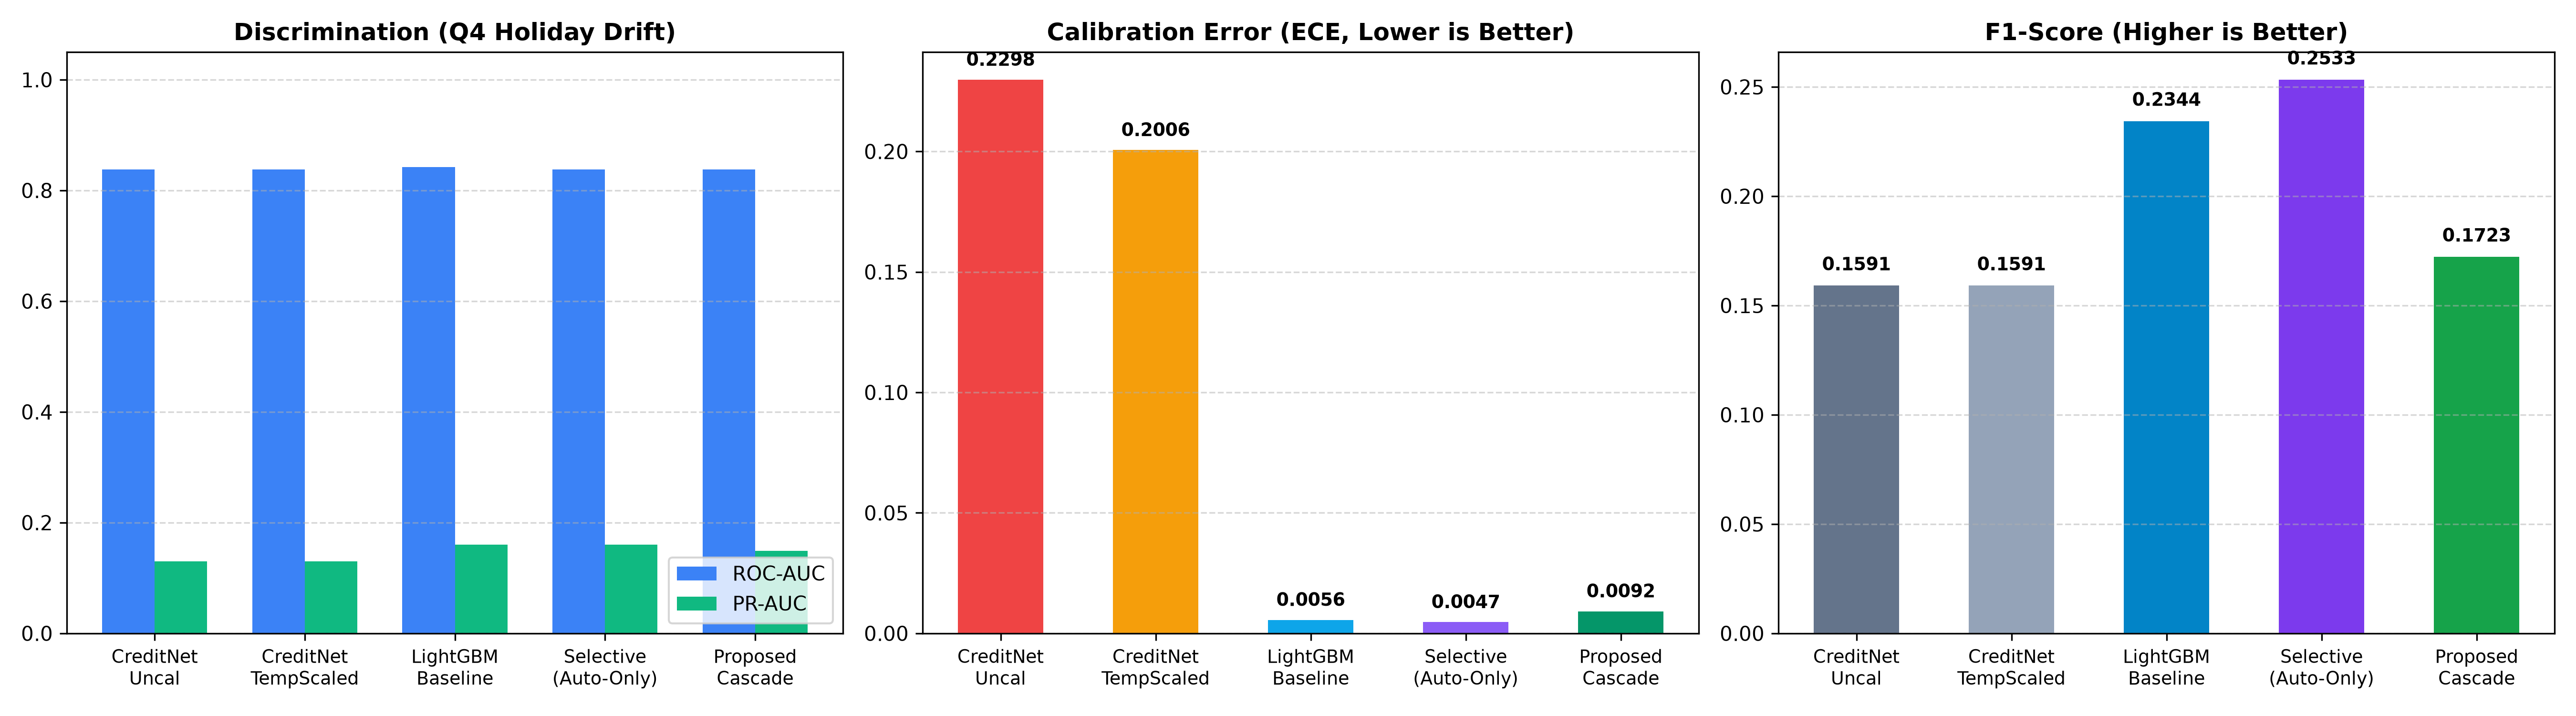
\includegraphics[width=0.92\textwidth]{experiments/results_2026/cascade_performance_comparison.png}
  \caption{Performance, calibration (ECE), and silent false-negative comparison across the five evaluated architectures.}
  \label{fig:cascade_comparison}
\end{figure*}

% ==============================================================================
% 7. LIVE GEMINI LLM AUDIT AND ERROR ANALYSIS (Target: ~1.5 columns + Table 3)
% ==============================================================================
\section{Live LLM Audit and Qualitative Analysis}

% TODO [WRITE IN YOUR OWN WORDS - Paragraph 1: 40-Case Live Evaluation]:
% Report sampling 40 cases (15 frauds, 25 legit) from 789 ambiguous test cases in [0.05, 0.11] using gemini-3.5-flash-lite.
% Report legitimate clearance: 18/25 (72.0% overall; 18/21 = 85.7% excluding 4 >10s API timeout fallbacks).

% TODO [WRITE IN YOUR OWN WORDS - Paragraph 2: Base-Rate Anchoring & Latency]:
% Explain low live recall (TP=1, FN=14, Recall=0.0667): Gemini anchored on 5%-10% System-1 probabilities without knowing the 2.06% base rate.
% Report latencies: 1.43 s avg on 36 successful calls (2.675 s overall with 4 timeouts), confirming 146.35 ms projected amortized cascade latency vs ~7 hours for 100% LLM.

% TODO [WRITE IN YOUR OWN WORDS - Paragraph 3: Case Studies]:
% Paraphrase 1 TP (TXN-00094695, $273.33, 10,354 km, 3 tx/1h -> FRAUD_CONFIRMED, 0.85) and 1 TN (TXN-00084969, $31.01 streaming -> LEGITIMATE_CLEARED, 0.065).

\begin{table}[t]
  \centering
  \caption{Live \texttt{gemini-3.5-flash-lite} audit summary on $N = 40$ ambiguous test transactions.}
  \label{tab:gemini_live}
  \resizebox{\linewidth}{!}{%
  \begin{tabular}{lc}
    \toprule
    \textbf{Metric} & \textbf{Observed Value} \\
    \midrule
    Sample Size ($N_{\text{fraud}} / N_{\text{legit}}$) & 40 (15 / 25) \\
    Confusion Matrix (TP / FP / TN / FN) & 1 / 7 / 18 / 14 \\
    API Timeouts ($>10\text{ s}$ Fallback to Proxy) & 4 / 40 (accounted for 4 of 7 FPs) \\
    Legitimate Clearance Rate (All / Non-Timeout) & 18/25 (72.0\%) / 18/21 (85.7\%) \\
    Accuracy / Precision / Recall / F1 & 0.4750 / 0.1250 / 0.0667 / 0.0870 \\
    Avg Latency (Non-Timeout / Overall) & 1.43 s / 2.675 s \\
    \bottomrule
  \end{tabular}}
\end{table}

% ==============================================================================
% 8. LIMITATIONS AND RESPONSIBLE AI DISCUSSION (Target: ~0.8 - 1.0 column)
% ==============================================================================
\section{Limitations and Responsible AI Considerations}

% TODO [WRITE IN YOUR OWN WORDS]:
% Discuss: (1) Base-rate anchoring in off-the-shelf LLMs; (2) API timeouts (4/40) requiring async System-2 queues; (3) Offline rule-proxy false-positive tradeoff (995 FPs); (4) Future calibration of LLM prompts with explicit class-prior context.

% ==============================================================================
% 9. CONCLUSION (Target: ~0.5 column)
% ==============================================================================
\section{Conclusion}

% TODO [WRITE IN YOUR OWN WORDS]:
% Summarize main findings: 90.27% automation at 17.3 ms single-tx latency, 0.0047 ECE, and modular System-2 auditing.

% ==============================================================================
% REFERENCES (Target: ~0.5 - 0.8 column)
% ==============================================================================
\begin{thebibliography}{9}

\bibitem{guo2017}
C.~Guo, G.~Pleiss, Y.~Sun, and K.~Q. Weinberger. 2017.
On Calibration of Modern Neural Networks.
In \textit{Proceedings of the 34th International Conference on Machine Learning (ICML)}.

\bibitem{gal2016}
Y.~Gal and Z.~Ghahramani. 2016.
Dropout as a Bayesian Approximation: Representing Model Uncertainty in Deep Learning.
In \textit{Proceedings of the 33rd International Conference on Machine Learning (ICML)}.

\bibitem{geifman2017}
Y.~Geifman and R.~El-Yaniv. 2017.
Selective Classification for Deep Neural Networks.
In \textit{Advances in Neural Information Processing Systems (NeurIPS)}.

\bibitem{hendrycks2017}
D.~Hendrycks and K.~Gimpel. 2017.
A Baseline for Detecting Misclassified and Out-of-Distribution Examples in Neural Networks.
In \textit{International Conference on Learning Representations (ICLR)}.

\bibitem{amodei2016}
D.~Amodei, C.~Olah, J.~Steinhardt, P.~Christiano, J.~Schulman, and D.~Man{\'e}. 2016.
Concrete Problems in AI Safety.
\textit{arXiv preprint arXiv:1606.06565}.

\bibitem{lin2026}
C.~Lin, Y.~Zhang, M.~Ran, W.~Xue, H.~Fan, Y.~Xu, Z.~Wan, S.~Han, Y.~Guo, and J.~Song. 2026.
Reinforcement Learning of Large Language Models for Interpretable Credit Card Fraud Detection.
\textit{arXiv preprint arXiv:2601.05578}.

\end{thebibliography}

\end{document}
